\documentclass[11pt]{beamer}

\mode<presentation>
{
  \usetheme{Edinburgh}
  \usefonttheme{structurebold}
}


\setbeamertemplate{section page}
{
    \begin{centering}
    \begin{beamercolorbox}[sep=12pt,center]{part title}
    \usebeamerfont{section title}\insertsection\par
    \end{beamercolorbox}
    \end{centering}
}
\usepackage{ifthen}
\usepackage{ucs}
% \usepackage[utf8x]{inputenc}

\usepackage[english]{babel}
\usepackage[latin1]{inputenc}
\usepackage{amsmath}
\usepackage{amssymb}
\usepackage{color,xcolor}
\usepackage{pifont}% http://ctan.org/pkg/pifont
\usepackage{times}
\usepackage[T1]{fontenc}
\usepackage{ulem}
\usepackage{graphicx}\graphicspath{{../figures/}} 
% \usepackage{media9}
% % \addmediapath{Movies/}
\usepackage{subfigure}
\usepackage{tikz}   
\usepackage{epstopdf}
\usepackage{caption}
\captionsetup{font=scriptsize,labelfont=scriptsize}
% \usepackage{multimedia}
\usepackage{movie15}
\usepackage{epstopdf}
\usepackage[]{color}
\usepackage{geometry}
\setbeamertemplate{navigation symbols}{}
\hypersetup
{
	pdftitle = {DLS Annual Meeting 2017},
	pdfauthor = {Andreea R\unichar{259}dulescu},
	pdfsubject = {},
	pdfkeywords = {},
	pdftoolbar = true,
	colorlinks = true,
	linkcolor = black,
	citecolor = green,
	urlcolor = black,
}


\usepackage{tikz}
\usetikzlibrary{decorations.pathreplacing,calc}
\newcommand{\tikzmark}[1]{\tikz[overlay,remember picture] \node (#1) {};}
\usepackage[percent]{overpic}

\newcommand{\signum}{\operatorname{sign}}
% \newcommand{\mbf}{\mathbf}
\newcommand{\mbb}{\mathbb}
\newcommand{\bsm}{\boldsymbol}
\newcommand{\mcl}{\mathcal}
\newcommand{\msf}{\mathsf}
\newcommand{\wtl}{\widetilde}
\newcommand{\wht}{\widehat}

\newcommand{\lit}[1]{{\color{white!45!black}\small~~(#1)}}
\newcommand{\red}[1]{{\color{red}#1}}
\newcommand{\hide}[1]{}
\renewcommand*{\thesubfigure}{}
\newcommand{\circled}[1]{\tikz[baseline=(char.base)]{\node[shape=circle,draw,inner sep=1pt] (char) {#1};}}
% Slightly reduce margin
\setbeamersize{text margin left=0.75cm}
\setbeamersize{text margin right=0.75cm}

\input{symbols}
\input{mathhdr}


\setbeamerfont{title}{series=\normalfont,size=\LARGE}
% \setbeamerfont{title in sidebar}{series=\bfseries}
% \setbeamerfont{author in sidebar}{series=\bfseries}
\setbeamerfont{author in head/foot}{series=\bfseries}
\setbeamerfont*{item}{series=}
\setbeamerfont{frametitle}{size=}
% \setbeamerfont{block title}{size=\small}
\setbeamerfont{subtitle}{size=\normalsize,series=\normalfont}
\setbeamertemplate{title page}
{
	{\usebeamercolor[fg]{title}\usebeamerfont{title}\inserttitle\par}
	\ifx\insertsubtitle\@empty
	\else
	\vskip0.25em
	{\raggedleft\insertsubtitle\par}
	\fi

% 	\vspace{2.5em}
% 	\includegraphics[width=0.6\textwidth]{figs/Dog2.jpeg}

	\vspace{2.em}
	\leftskip=0pt plus1fill\textbf{\insertauthor}\par
	\vspace{1.em}

% 	\insertinstitute\vskip1em
	\usebeamerfont{institute}{\tiny \insertinstitute}\par
	\begin{center}
	\includegraphics[width=1.5cm]{iit_advr.png}
	\hspace*{6mm}
	\includegraphics[width=4.5cm]{idiap_logo.png}
	\hspace*{6mm}
	\includegraphics[width=1.5cm]{oxford_logo.png}

% 	\hspace*{90mm}
	\end{center}
	\vspace{-2.5em}
% 	{\raggedleft\insertdate\par}

}
% \setbeamertemplate{sidebar right}
% {
% 	\vskip0.5em
% 	\hbox to 1.75cm{\hss\insertlogo\hss}
% 	\vskip0.5em
% 	\insertverticalnavigation{2cm}%
% 	\vfill
% 	\hbox to 2cm{\hfill\usebeamerfont{subsection in
% 		sidebar}\strut\usebeamercolor[fg]{subsection in
% 		sidebar}\insertframenumber\hskip5pt}
% 	\vskip1.5pt
% }

\setbeamertemplate{footline}
{
	\leavevmode
	\hbox{
		\begin{beamercolorbox}[wd=0.45\paperwidth,ht=2.25ex,dp=2ex,center]{author
			in head/foot}
			\usebeamerfont{author in head/foot}
			\insertshortauthor\hspace{1em}\insertshortinstitute
		\end{beamercolorbox}
		\begin{beamercolorbox}[wd=0.4\paperwidth,ht=2.25ex,dp=2ex,center]{title
			in head/foot}
			\usebeamerfont{title in head/foot}\insertshorttitle
		\end{beamercolorbox}
		\begin{beamercolorbox}[wd=0.15\paperwidth,ht=2.25ex,dp=2ex,center]{date in
			head/foot}
			\insertframenumber{} / \inserttotalframenumber\hspace*{2ex} 
		\end{beamercolorbox}
	}
  \vskip0pt
}




\title[\color{white} Whole-body Trajectory Optimization]{Whole-body Trajectory Optimization for Non-periodic Dynamic Motions on Quadrupedal Systems}

% Author: [argument in brackets] appears at the bottom of all slides
\author[Andreea R\unichar{259}dulescu]{Andreea R\unichar{259}dulescu$^{1}$  Ioannis Havoutis$^{2,3}$ Darwin G. Caldwell$^1$ Claudio Semini$^{1}$}


% % This talk will give an overview of the previously developed optimal control framework for robotic systems in domains with contacts possesing impedance modulation capabilities.
% % I will introduce the motivation for model accuracy improvement and present the selected methodology for learning dynamics. The current state of the investigation and issues encountered will be 
% % described.

% Institute: [argument in brackets] as above
\institute[]{$^{1}$Dynamic Legged Systems Lab., Department of Advanced Robotics, Istituto Italiano di Tecnologia, Genova, Italy \\
$^{2}$Robot Learning and Interaction Group, Idiap Research Institute, Martigny, Switzerland \\
$^{3}$Oxford Robotics Institute, Department of Engineering Science, University of Oxford, United Kingdom
}

\date{March 16th, 2017}
% \date{\today}

%%%%%%%%%%%%%%%% Useful commands %%%%%%%%%%%%%%%%

\newcommand\CopyrightText[1]{%
  \begin{textblock*}{\paperwidth}(0\paperwidth,.97\paperheight)%
    \hfill\textcolor{white}{\tiny#1}\hspace{3pt}
  \end{textblock*}
}

\newcommand{\citeFoot}[1]
{
    \rule{\linewidth}{0.5pt}
    {\scriptsize #1}
}

\newcommand{\fullFrameImage}[2]
{
    {
        \usebackgroundtemplate{\includegraphics[height=\paperheight]{#1}}
        \frame[plain]
        {
            \CopyrightText{ #2}
        }
    }
}

\newcommand{\fullFrameMovie}[2]
{
    {
        \setbeamertemplate{background canvas}[vertical shading][bottom=black,top=black]
        %\setbeamercolor{background canvas}{bg=black}

        \frame[plain]
        {
            \begin{textblock*}{\paperwidth}(0px,0px)%
            \flashmovie[width=\paperwidth,height=0.96\paperheight,engine=flv-player,auto=1,controlbar=0]{#1}
            \end{textblock*}
            \CopyrightText{#2}
        }
        
    }
}

\newcommand{\blackframe}
{
    {
        \setbeamertemplate{background canvas}[vertical shading][bottom=black,top=black]
        \frame[plane]{}
        \addtocounter{framenumber}{-1}
    }
}

%%%%%%%%%%%%%%%% End useful commands %%%%%%%%%%%%%%%%

\usepackage{media9}%
% \renewcommand{\includemovie}[3]{%
% \includemedia[%
% width=#1,height=#2,%
% activate=pagevisible,%
% deactivate=pageclose,%
% addresource=#3,%
% flashvars={%
% src=#3 % same path as in addresource!
% &autoPlay=true % default: false; if =true, automatically starts playback after activation (see option ‘activation)’
% &loop=true % if loop=true, media is played in a loop
% &controlBarAutoHideTimeout=0 %  time span before auto-hide
% }%
% ]{}{/usr/local/share/texmf/media9/players/StrobeMediaPalyback.swf}%
% }
\begin{document}

 \begin{frame}
  \titlepage
%   \vspace*{-5mm}
%   \begin{figure}[h!]
%   \includegraphics[scale=.25]{iitlogo.png} 
%   \end{figure}
\end{frame}

\begin{frame}\frametitle{\color{black} Introduction}

     \begin{itemize}\small \addtolength{\itemsep}{0.1ex}
     \item biological legged systems $\rightarrow$ whole body movements
     \item high performance despite noise in biological motor systems
     \end{itemize}
 
%     \begin{figure}[h!]
%     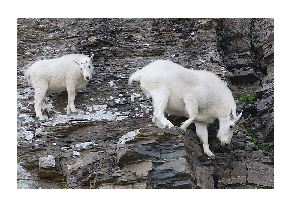
\includegraphics[scale=.72]{mountaingoat.eps} 
%     \hspace*{15mm}
% %     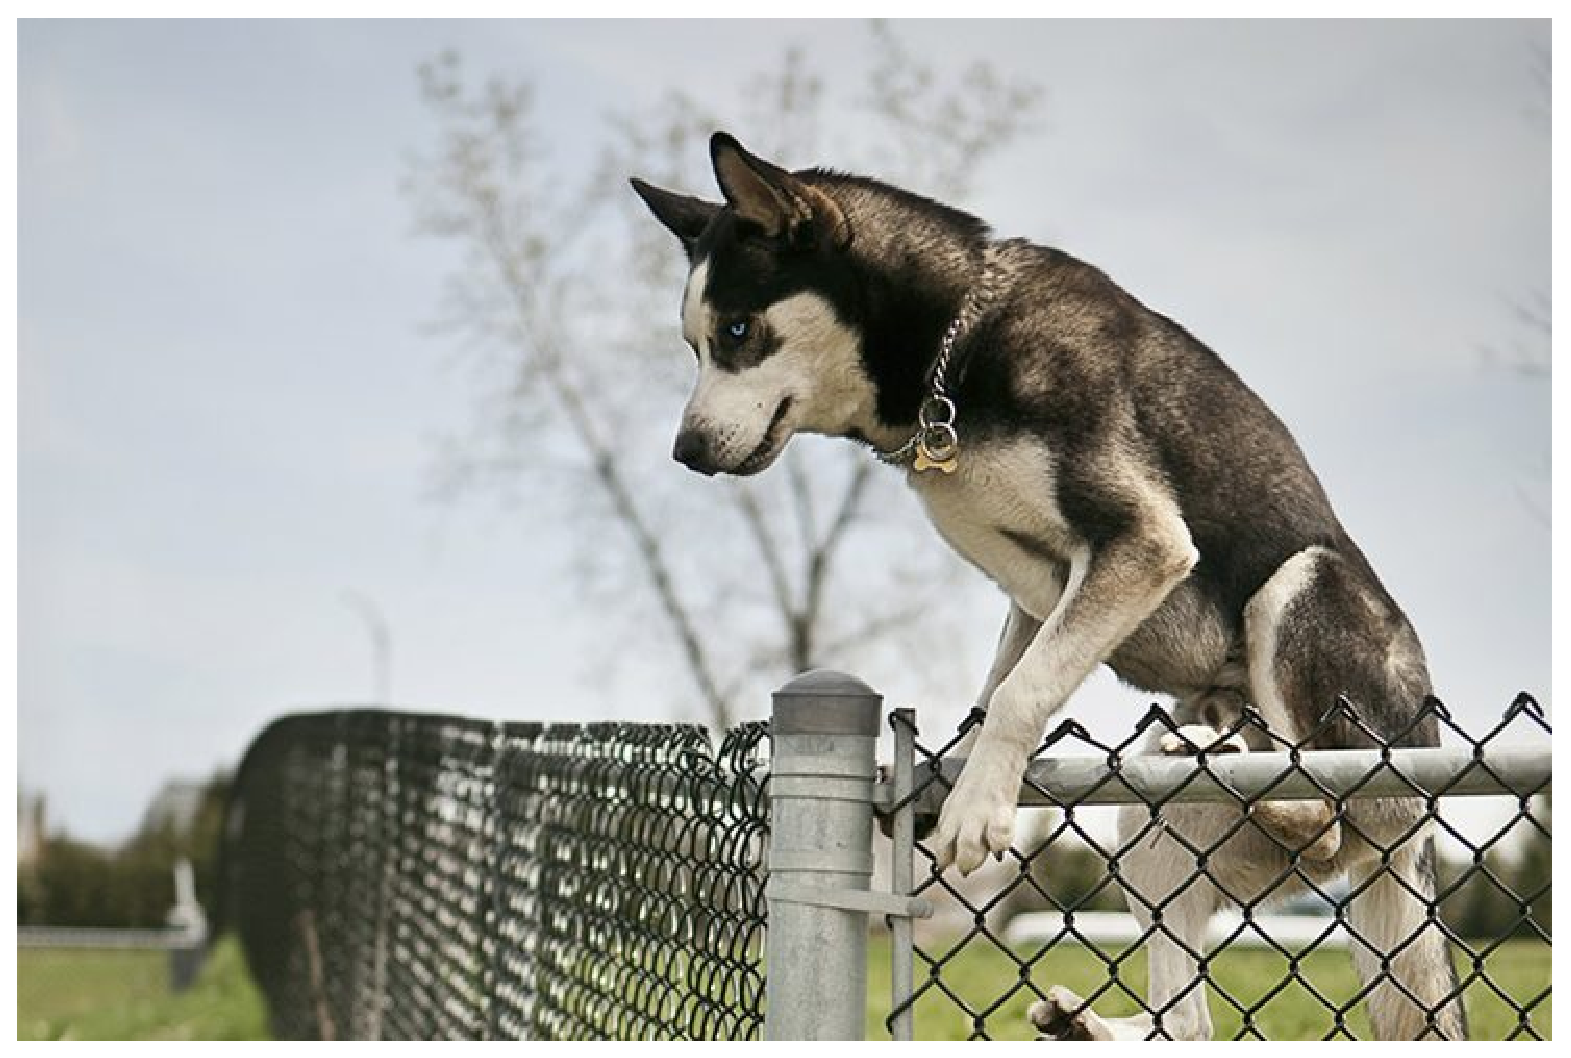
\includegraphics[scale=.12]{fencedog.eps}
%     \includegraphics[scale=.055]{parkour_dog.jpg}
%     \end{figure}
\vspace*{-5mm}
\begin{columns}
\column{.46\textwidth}
\begin{center}
\includemedia[ width=0.7\linewidth, activate=pagevisible, deactivate=onclick, 
  addresource=Movies/goat_parkour.m4v,
  flashvars={source=Movies/goat_parkour.m4v
  &loop=true
  &autoPlay=true}]
  {{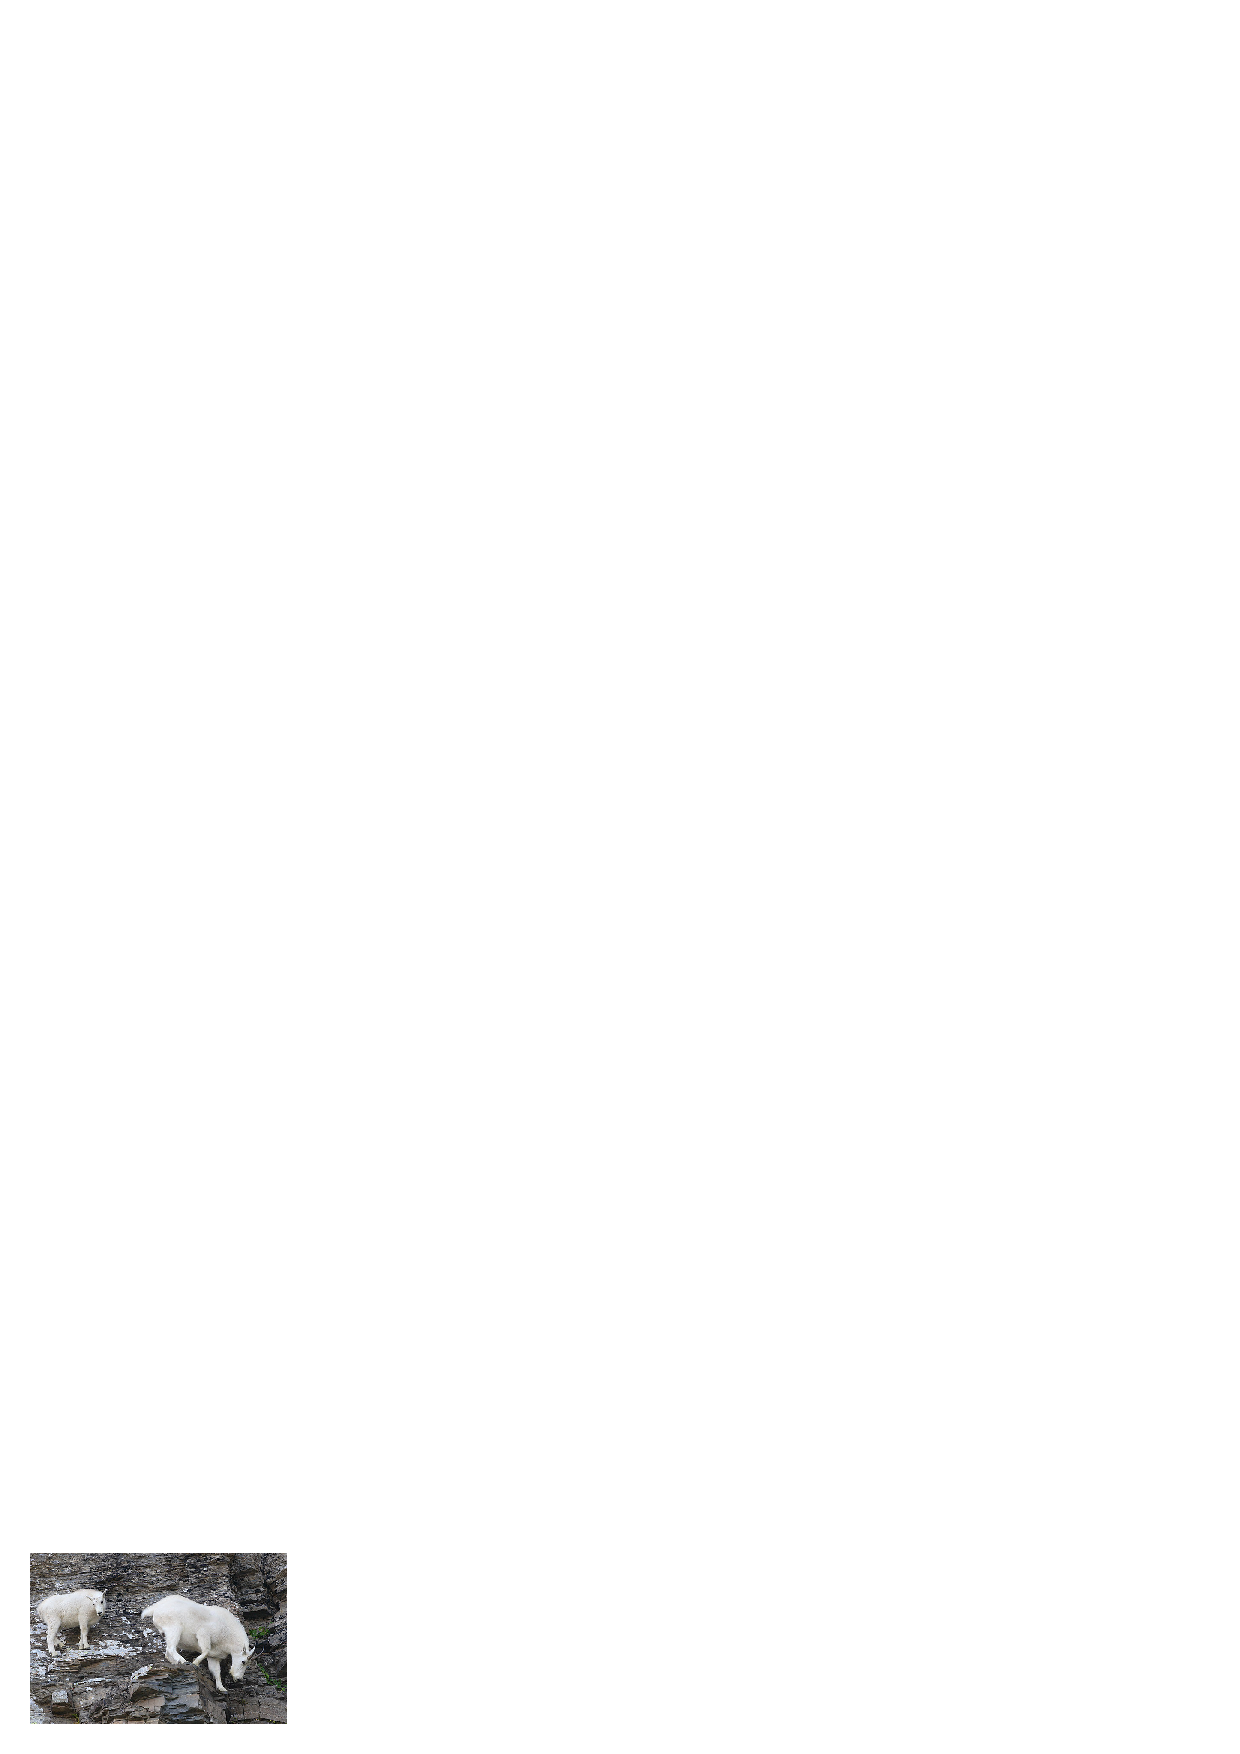
\includegraphics[width=0.7\linewidth]{mountaingoat.jpg}}}{media9/players/VPlayer9.swf}
\end{center}   
\column{.54\textwidth} 
\begin{center}
\includemedia[ width=0.7\linewidth, activate=pagevisible, deactivate=onclick,
  addresource=Movies/dog_parkour_short.m4v,
  flashvars={source=Movies/dog_parkour_short.m4v
  &loop=true
  &autoPlay=true}]
  {{\includegraphics[width=0.7\linewidth]{parkour_dog.jpg}}}{media9/players/VPlayer9.swf} 
\end{center}   
\end{columns}

%     \pause
     \begin{itemize}\small \addtolength{\itemsep}{0.1ex}
%      \item most robotic legged research: periodic tasks   
      \item legged systems $\rightarrow$ multiple contact events 
      \item optimization and learning approaches (MPC, $PI^{2}$, CMA)
      \item most robotic legged research: periodic tasks  
      (use task/domain specific knowledge, predefined heuristics, teleoperation) 
%       \item fully autonomous systems: non-periodic tasks    
%       \item little generalised approaches for self-righting (vs. fall avoidance)
     \end{itemize}
     
  \begin{figure}
  \centering
  \hspace*{-5mm}
  \includegraphics[scale=.14]{feet_sequence.png}
  \includegraphics[scale=.14]{mit_teleop.jpg}
  \includegraphics[scale=.14]{sr_robot_general.jpg} 
  \end{figure}
  \end{frame}

\begin{frame}\frametitle{\color{black} Trajectory Optimization for Non-periodic Dynamic Motions}
%  Overview:
 \begin{itemize} \addtolength{\itemsep}{0.5ex}
  \item generalised approach $\rightarrow$ whole body movement solutions
 \end{itemize}
 \pause
 
   \begin{itemize}\small
   \item finding the appropriate joint motions for each given task
   \item direct optimisation(joints/torques): large search space
   \item parametrised policy (weighted average of Gaussian kernels)
  \end{itemize}

 \begin{equation}\nonumber
  f(t)  = \sum_{i=1}^{M} w_i \phi_i(t)/ \sum_{i=1}^{M} \phi_i(t), \; \phi_i(t) = 
exp(- \frac{1}{2 \sigma^2} (t-\mu_i))
  \end{equation} 
 \pause
  \begin{minipage}[t]{0.48\linewidth}
  \vspace*{15mm}
  \begin{center}
     Covariance Matrix Adaptation \\ Evolution Strategy (CMA-ES)  \\
      $\downarrow$ \\
      $ w_i, \; i = 0 \cdots M$ $\rightarrow$
        \end{center}
  \end{minipage}\hfill
  \begin{minipage}[t]{0.48\linewidth}
    \begin{figure}[h!]
  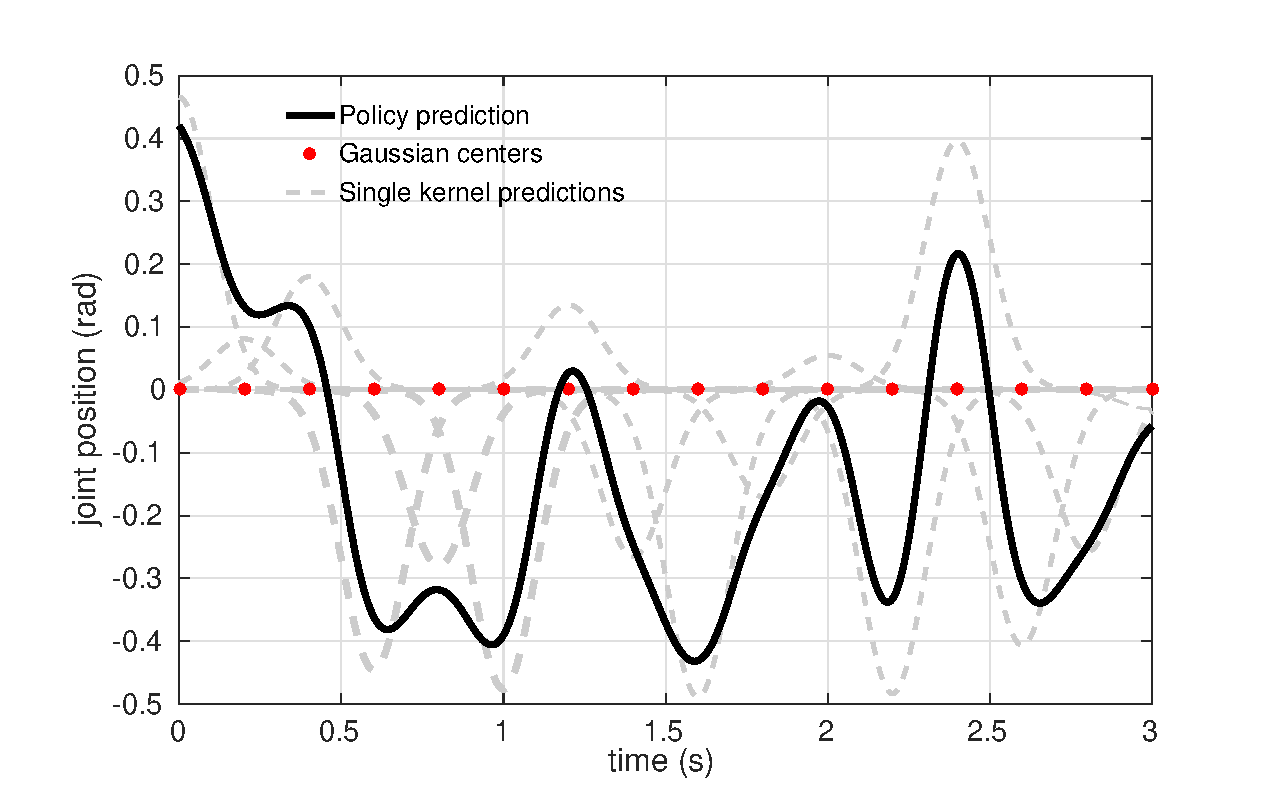
\includegraphics[scale=.3]{example_gr2.eps} 
  \end{figure}\end{minipage}
    
\end{frame}

\begin{frame}\frametitle{\color{black} Experimental setup}

  \begin{itemize}\small
  \item realistic simulation of the HyQ2Max quadrupedal robot
%   \item features 12 hydraulically actuated joints 
  \item each limb has 3 actuators: HAA (hip abduction/adduction), HFE (hip 
flexion/extension) and KFE (knee flexion/extension)
 \end{itemize}
  \vspace*{-5mm}
 \begin{figure}
  \centering
  \includegraphics[scale=.34]{hyq2max_whiteBG.jpg}
  \hspace*{7mm}
  \includegraphics[scale=.03]{hyq2max_cad.jpg}
 \end{figure}
 \vspace*{-5mm}
  \begin{itemize}\small
   \item we use 12 policies, one for each joint
   \item $M=16$ Gaussian kernels, means equally spaced, $\sigma^2 = 0.01$
  \end{itemize}

\end{frame}


\begin{frame}\frametitle{\color{black} Rearing}
  \begin{itemize}\small
  \item the system is in a neutral/standard configuration
  \item task: bring the system to a rearing pose (desired \textit{torso pitch} and \textit{torso CoM 
(center of mass) height})
%   \item front and back leg pairs share the same policies
 \pause
  \item result: 177 evaluation eps. - 17 samples/ep.
 \end{itemize}
 
 \vspace*{-5mm}
 \begin{figure}
 \centering
%  \hspace*{-3mm}
%  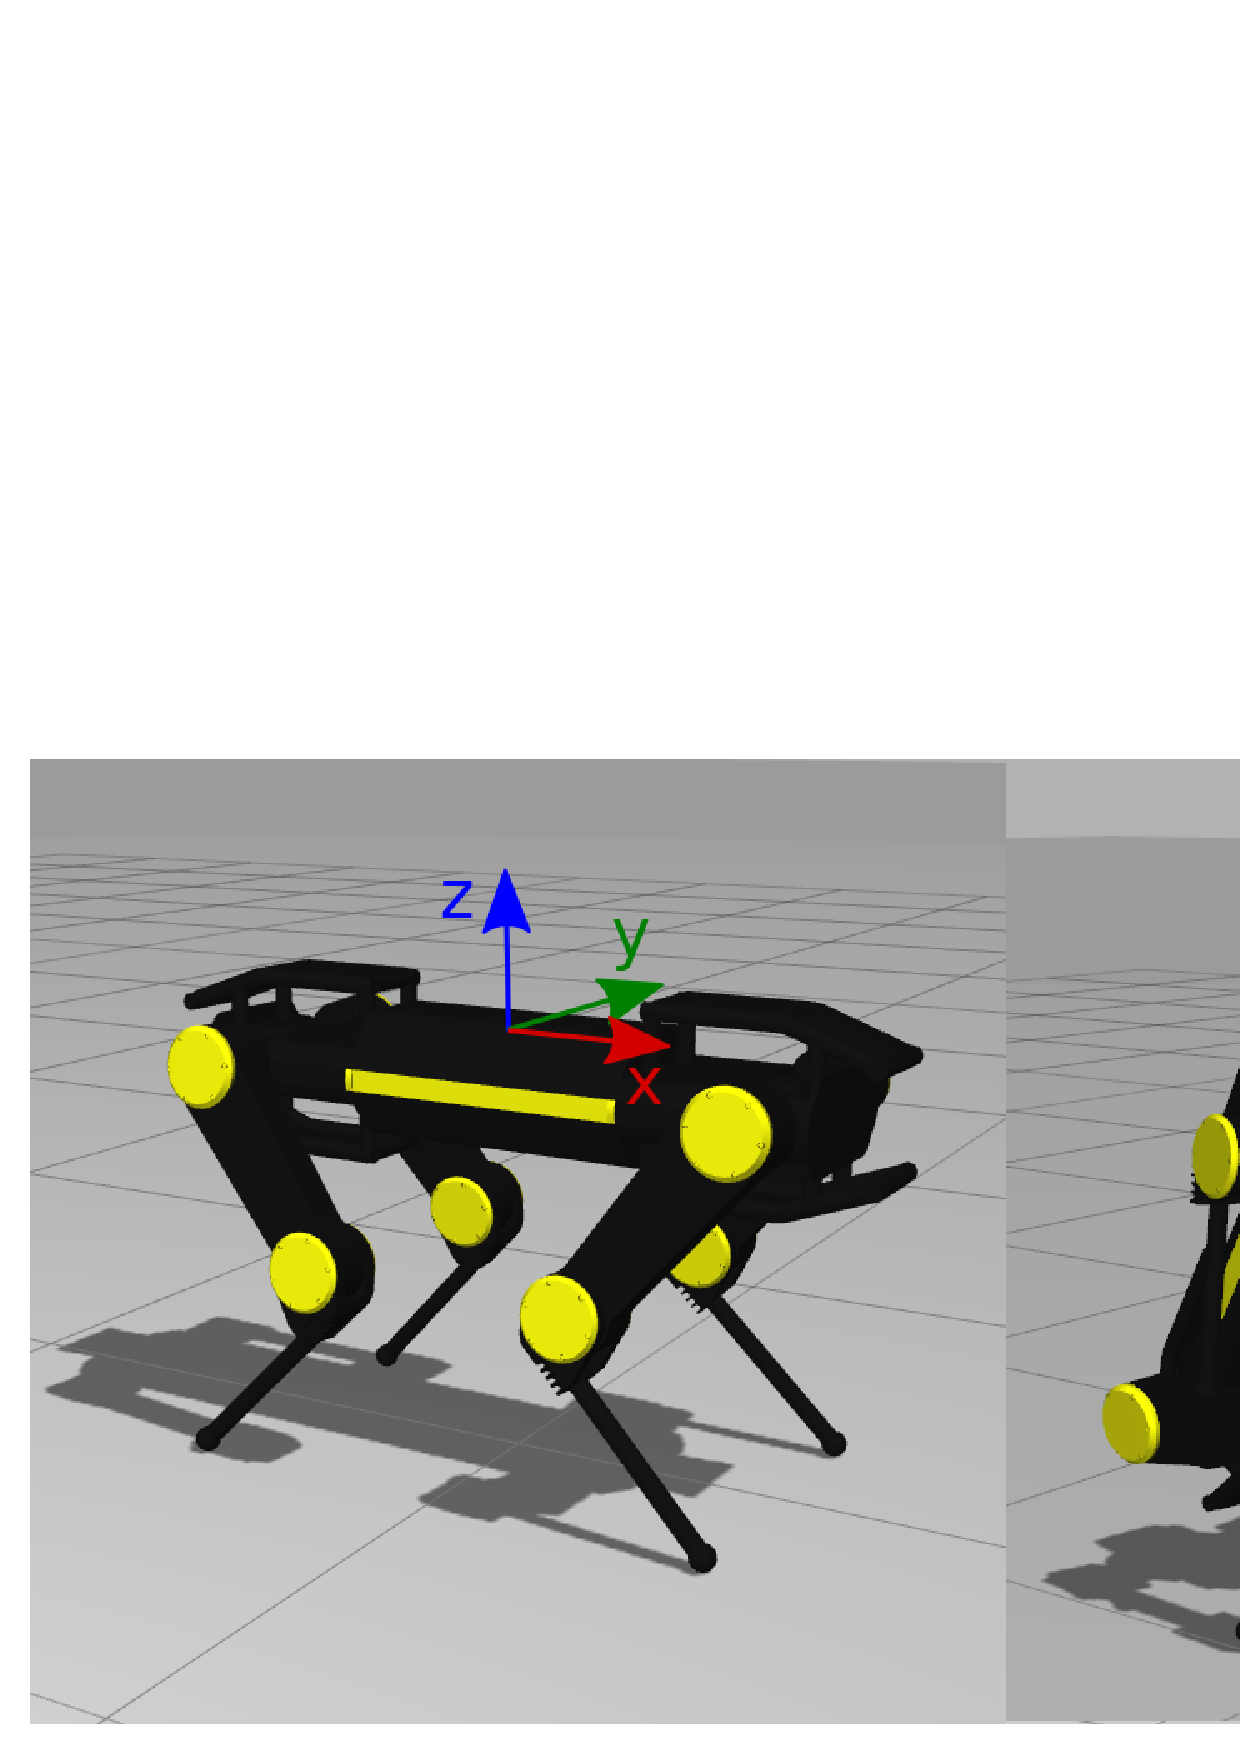
\includegraphics[scale=.2]{rearing_befor_after_ins.png} 
\includemedia[
  width=0.37\linewidth,
  height=0.25\linewidth,
  activate=onclick,
  deactivate=onclick,
  addresource=Movies/RearingExplore_25May_3.m4v,
  flashvars={source=Movies/RearingExplore_25May_3.m4v
%   &loop=true
%   &autoPlay=true
  }]
  {{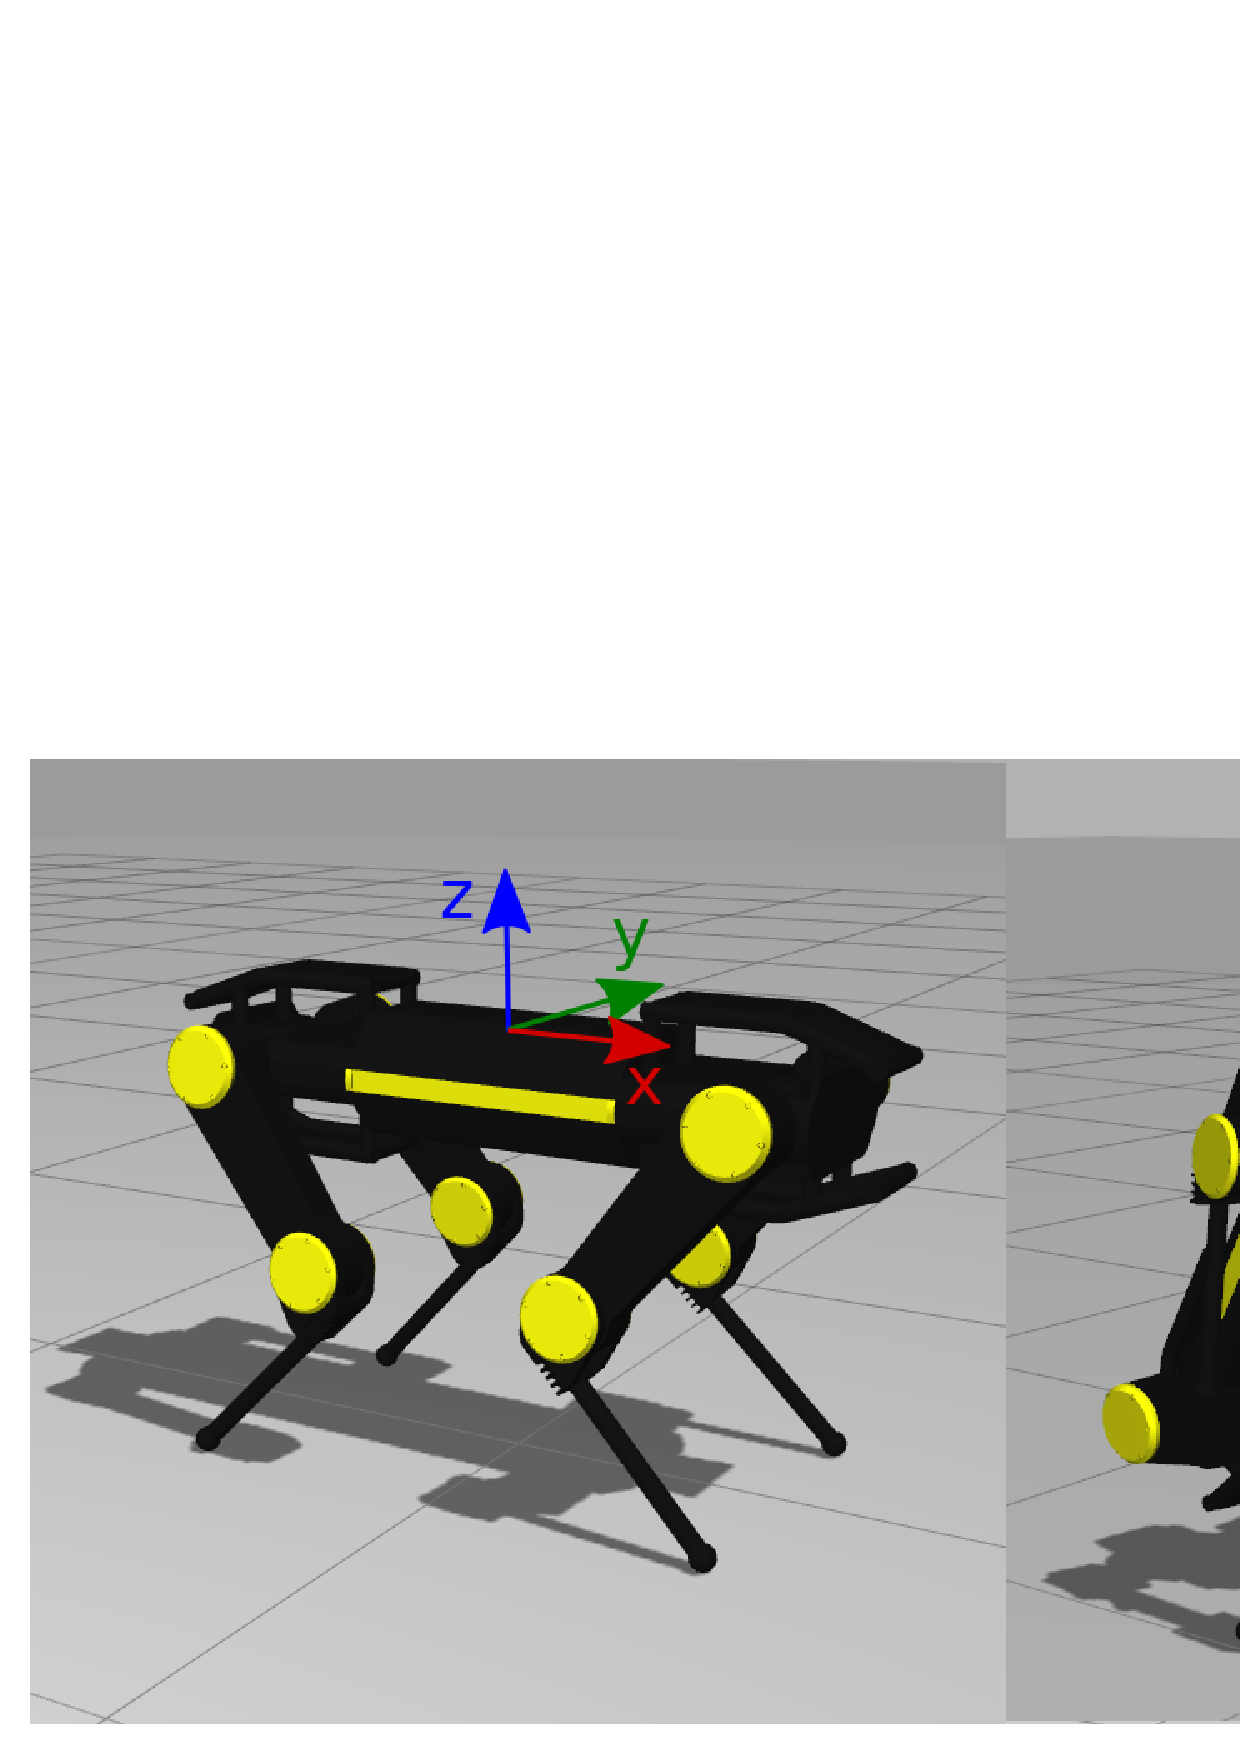
\includegraphics[width=0.37\linewidth, height=0.25\linewidth]{rearing_befor_after_ins.png}}}{media9/players/VPlayer9.swf}
%  \hspace*{3mm}
 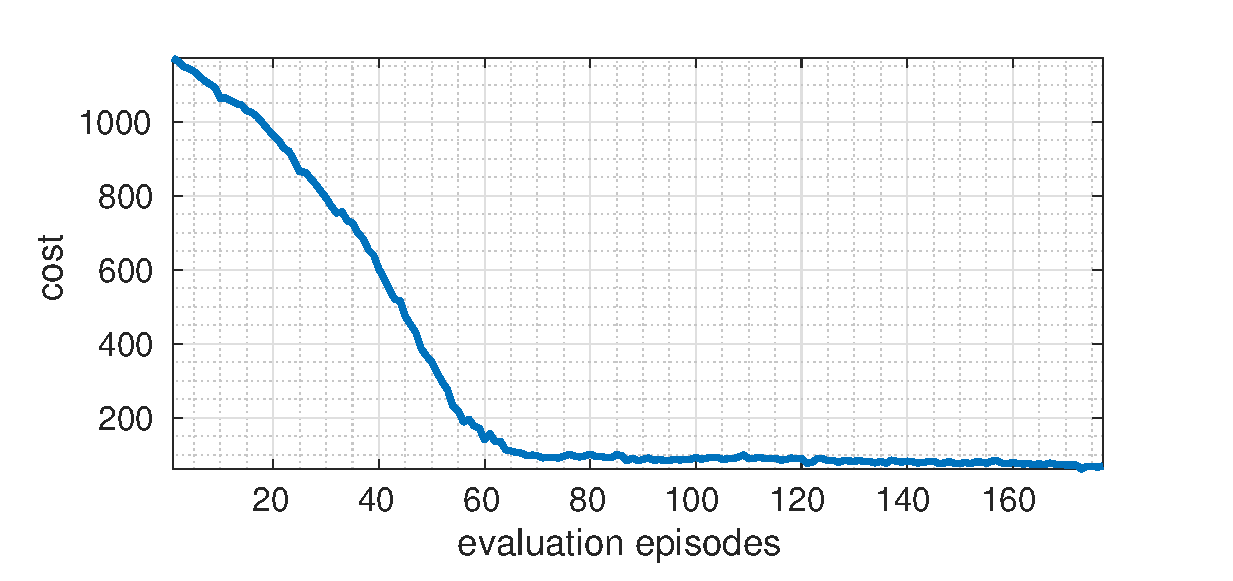
\includegraphics[scale=.32]{sr_cost_1_ICRA.eps} 
 \end{figure}
 
\end{frame}

\begin{frame}\frametitle{\color{black} Pose recovery}
 \begin{itemize}\small
  \item regular locomotion task fails, unexpected state
  \item task: return to a \textit{neutral orientation, desired torso 
CoM height}
%   \pause
  \item result: 158 evaluation eps. - 19 samples/ep.
 \end{itemize}
 
%  \begin{figure}
%  \centering
%  \hspace*{-5mm}
%  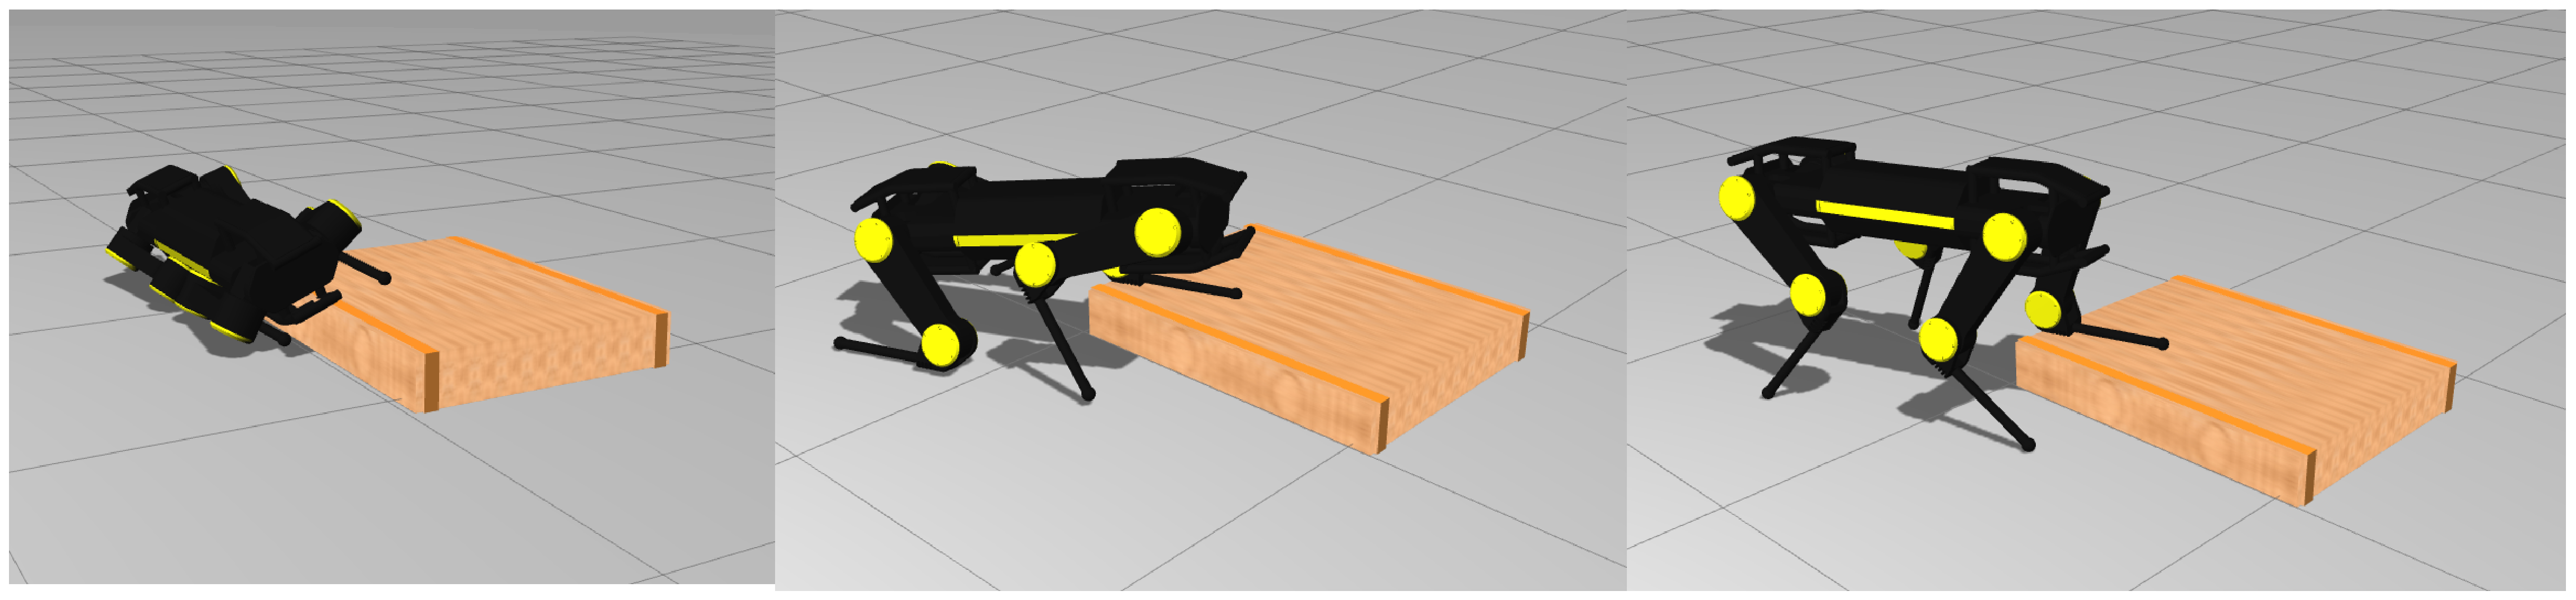
\includegraphics[scale=.14]{sr_befor_after.eps} 
%  \end{figure}
%  
%  \begin{center} 
% \href{run:Movies/icra17aradulescu_final.mp4}{\beamerbutton{video}}
% \end{center}
\vspace*{-5mm}
\begin{center}
% \movie[height = 0.6\textwidth, width = 0.8\textwidth, poster, showcontrols]{}{Movies/trimmed_poseRec_ICRA17.mp4}
% \includemovie{.85\textheight}{.85\textheight}{Movies/trimmed_poseRec_ICRA17.flv}%
\includemedia[
  width=0.75\linewidth,
  height=0.55\linewidth,
  activate=pagevisible,
  deactivate=onclick,
  addresource=Movies/trimmed_poseRec_ICRA17.mp4,
  flashvars={source=Movies/trimmed_poseRec_ICRA17.mp4
  &loop=true
  &autoPlay=true}]
  {{\includegraphics[width=0.75\linewidth, height=0.55\linewidth]{sr_after.png}}}{media9/players/VPlayer9.swf}

\end{center} 
\end{frame}

% \begin{frame}\frametitle{\color{black} Video}
% 
% \begin{block}{Test Video}
% 
% \begin{center}
% \movie[height = 0.6\textwidth, width = 0.8\textwidth, poster, showcontrols] {}{Movies/icra17aradulescu_final.mp4}
% \end{center} 
% 
% \end{block}
%  
% \end{frame}


\begin{frame}\frametitle{\color{black} Final remarks}
  \begin{block}{Overview}
    \begin{itemize}\addtolength{\itemsep}{0.1ex}
      \item whole body optimisation for non-periodic dynamic movements
%       \item non-periodic dynamic movements on quadrupedal systems
      \item trajectory solutions involving multiple contacts
      \item without any predefined feet placement heuristics
%       \item high level goals encoded in the cost function
    \end{itemize} 
  \end{block}
  
    \begin{block}{Future directions}
     \begin{itemize}\addtolength{\itemsep}{0.1ex}
      \item transfer the obtained behaviours onto the hardware system
      \item autonomous initial phase detection and desired final goal 
      \item expand the range of motions (e.g., self-righting)
%       \item learning based on a motion library
     \end{itemize}
    \end{block}

\end{frame}


\begin{frame}
\vspace*{-7mm}
 	\begin{center}
		\LARGE Thank you for your attention. \\
	\end{center}
	\vspace*{5mm}
	\begin{center}
		\LARGE See you at {\color{red} Booth $\#4$} \\
	\end{center}
% 	
% \footnotesize \textbf{Development team:}\\
% Alex Posatskiy\\
% Antonios Gkikakis\\
% Carlos Mastalli\\
% Claudio Semini\\
% Darwin G. Caldwell\\
% Dhinesh Sangiah\\
% Ioannis Havoutis\\
% Josephus Driessen\\
% Marco Camurri\\
% Marco Frigerio\\
% Michele Focchi\\
% Octavio Villarreal\\
% Romeo Orsolino\\
% Roy Featherstone\\
% Roodra Pratap Singh Bajwa\\
% Victor Barasuol\\
% Yannick Berdou\\
% Yifu Gao\\ 
\end{frame}

\end{document}